% Codice C
\begin{lstlisting}[language=C]
    
\end{lstlisting}

% Allineamento
\begin{align*}
    A = [a_0, a_1, a_{n - 1}] \\
    B = [b_0, b_1, b_{n - 1}]
\end{align*}

% Immagini
\begin{figure}[h!]
    \centering
    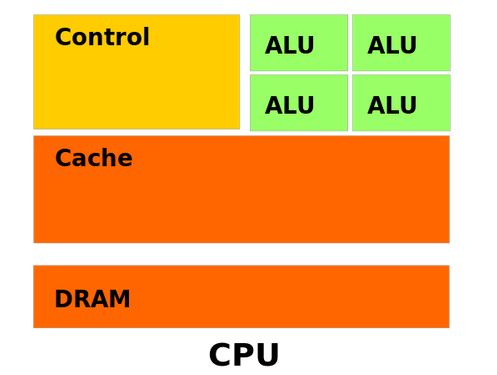
\includegraphics[scale=0.6]{img/CPU.png}
    \caption{Immagine dettagliata delle componenti di una CPU}
\end{figure}

% Algoritmo
\begin{algorithm}
    \caption{My algorithm}\label{alg:cap}
    \hspace*{\algorithmicindent} \textbf{Input} \\
    \hspace*{\algorithmicindent} \textbf{Output}
    \begin{algorithmic}[1]
        \State $y \gets 1$
        \State $X \gets x$
        \State $N \gets n$
        \While{$N \neq 0$}
        \If{$N$ is even}
            \State $X \gets X \times X$
            \State $N \gets \frac{N}{2}$  \Comment{This is a comment}
        \ElsIf{$N$ is odd}
            \State $y \gets y \times X$
            \State $N \gets N - 1$
        \EndIf
        \EndWhile
    \end{algorithmic}
\end{algorithm}

%% Matrici
\begin{equation}
    L_{Diff} = 
\begin{pmatrix}
    -2 & 1 & & & \\
    1 & -2 & 1 & \\
    & & \ddots & \ddots & & \\
    & & 1 & -2 & 1 \\
    & & & 1 & -2
 \end{pmatrix}
 \in \mathbb{R} ^ {M, M} \label{eq:Ldiff}
\end{equation}


\begin{equation}
    L = \frac{1}{\Delta x^2} 
\begin{pmatrix}
    L_{Diff} & 0 & 0 \\
    0 & DL_{Diff} & 0 \\
    0 & 0 & dL_{Diff}
 \end{pmatrix}
 \in \mathbb{R} ^ {3M, 3M} \label{eq:LMatrix}
\end{equation}

% Tabelle
\begin{table}[h!]
    \centering
    \begin{tabularx}{0.8\textwidth} { 
      | >{\centering\arraybackslash}X 
      | >{\centering\arraybackslash}X
      | >{\centering\arraybackslash}X
      | >{\centering\arraybackslash}X
      | >{\centering\arraybackslash}X|
    }
    \hline
     &  &  \\
    \hline  &  &  \\ 
    \hline  &  &  \\ 
    \hline  &  &  \\ 
    \hline  &  &  \\
    \hline  &  &  \\ 
    \hline
    \end{tabularx}
    \caption{Write a caption here}
    \label{tab:my_label}
\end{table}

%%%%%%%%%%%%%%%%%%%%%%%%%%%%%% Tabelle utili poi %%%%%%%%%%%%%%%%%%%%%%%%%%%

\newpage


\begin{table}[h!]
    \centering
    \begin{tabularx}{0.8\textwidth} { 
      | >{\centering\arraybackslash}X 
      | >{\centering\arraybackslash}X
      | >{\centering\arraybackslash}X
      | >{\centering\arraybackslash}X
      | >{\centering\arraybackslash}X|
    }
     \hline
     \textbf{M} & \textbf{Threads} & \textbf{Blocks} & \textbf{CPU time} (s) & \textbf{GPU time} (s) \\
     \hline
     4 & $2\times2$ & $2\times2$ & 0.000025 & 0.000617 \\ 
     \hline
     8 & $4\times4$ & $2\times2$ & 0.000039 & 0.000571 \\ 
     \hline
     16 & $8\times8$ & $2\times2$ & 0.000075 & 0.000610 \\ 
     \hline
     32 & $16\times16$ & $2\times2$ & 0.000201 & 0.000669 \\ 
     \hline
     64 & $16\times16$ & $4\times4$ & 0.000934 & 0.000948 \\ 
    \hline
    \end{tabularx}
    \caption{Tempi di esecuzione algoritmo parallelo e sequenziale per il calcolo della matrice $L$ all'aumentare di $M$}
    \label{tab:parseq1}
\end{table}


\begin{table}[h!]
    \centering
    \begin{tabularx}{0.8\textwidth} { 
      | >{\centering\arraybackslash}X 
      | >{\centering\arraybackslash}X
      | >{\centering\arraybackslash}X
      | >{\centering\arraybackslash}X
      | >{\centering\arraybackslash}X|
    }
    \hline
    \textbf{Threads} & \textbf{Blocks} & \textbf{GPU time} (s) \\
    \hline $2\times2$ & $32\times32$ & 0.000972 \\ 
    \hline $4\times4$ & $16\times16$ & 0.000958 \\ 
    \hline $8\times8$ & $8\times8$ & 0.000949 \\ 
    \hline $16\times16$ & $4\times4$ & 0.000948 \\
    \hline $32\times32$ & $2\times2$ & 0.001028 \\ 
    \hline
    \end{tabularx}
    \caption{Tempi di esecuzione $M = 64$ per il calcolo della matrice $L$ all'aumentare del numero di thread e blocchi}
    \label{tab:my_label}
\end{table}


%--------------------------------------------------------------
%       Tabelle dei tempi confronto GPU e CPU
%--------------------------------------------------------------
\newpage
\begin{table}[h!]
    \centering
    \begin{tabularx}{1\textwidth} { 
      | >{\centering\arraybackslash}X 
      | >{\centering\arraybackslash}X
      | >{\centering\arraybackslash}X
      | >{\centering\arraybackslash}X
      | >{\centering\arraybackslash}X
      | >{\centering\arraybackslash}X
      | >{\centering\arraybackslash}X|
    }
    \hline $\Delta _{t}$ & N & CPU time (s) & GPU time \\
    \hline $1 / 2^{11}$ & $102400 \approx 1 \times 10^5$  & 10.220000 & 1 \\ 
    \hline $1 / 2^{12}$ & $204800 \approx 2 \times 10^5$ & 20.120000 & 1 \\ 
    \hline $1 / 2^{13}$ & $409600  \approx 4 \times 10^5$  & 40.340000 & 1 \\ 
    \hline $1 / 2^{14}$ & $819200  \approx 8 \times 10^5$  & 81.740000 & 1 \\
    \hline $1 / 2^{15}$ & $1638400  \approx 1 \times 10^6$  & 170.340000 & 1 \\ 
    \hline $1 / 2^{16}$ & $3276800  \approx 3 \times 10^6$  & \text{Cannot allocate} & \text{Cannot allocate} \\
    \hline
    \end{tabularx}
    \caption{Confronto tempi dell'algoritmo sequenziale e parallelo per $M = 64$ e $N$ e $\Delta _{t}$ variabili} 
    \label{tab:cpu_gpu_time}
\end{table}

\vspace{0.2cm}





%%%%%%%%%%%%%%%%%%%%%%%%%%%%%%%%%%%%%%%%%%
% TABLE
%%%%%%%%%%%%%%%%%%%%%%%%%%%%%%%%%%%%%%%%%%
%\setlength{\arrayrulewidth}{0.5mm}
%\setlength{\tabcolsep}{10pt}

\begin{table}[ht!]
    \begin{center}
        \renewcommand{\arraystretch}{1.5}
        \begin{adjustbox}{width=1\textwidth}
            \begin{tabular}{ |c|c|c|c|c|c|c|c| }
                \hline
                \multicolumn{2}{|c}{} & \multicolumn{2}{|c}{computeYGPU} & \multicolumn{2}{|c|}{computeOneColumnGPU} & \multicolumn{2}{|c|}{Tempo totale modulo} \\
                \hline
                \textit{$\Delta _t$} & N & Chiamate & Tempo medio(s) & Chiamate & Tempo medio(s) & GPU(s) & CPU(s) \\
                
            \end{tabular}
        \end{adjustbox}
    \end{center}
    \caption{An example table.}
    \label{table:example_table}
\end{table}
